% !TEX TS-program = xelatex
% !TEX encoding = UTF-8 Unicode

\providecommand{\home}{../..}
\documentclass[\home/main.tex]{subfiles}

\begin{document}


% Dit hoort volgens mij eerder thuis in introductie:
%For example, a recent cloth folding pipeline by~\citeauthor{Doumanoglou2016} starts with a visual perception to detect candidate grasp points. These grasp points are then given to a planning module to move the robot end-effector to the desired position and orientation. This divide-and-conquer methodology leads to a loss of information between the different stages, resulting in the accumulation of errors. \Citeauthor{Doumanoglou2016} report difficulties when folding towels because the perception system labels them as shirts. These individual components are built in a laboratory environment with certain assumptions which are likely to be violated in an unstructured, complex environment. Inaccurate sensor readings together with deformation of the robot’s links also deteriorate the accuracy of these systems. In contrast, modern deep learning approaches try to achieve the same outcome in an end-to-end fashion. This is done by 

\chapter{introduction}\label{ch:introduction}
A patent in $1691$ heralded a change for millions of individuals unprivileged to having a team dedicated for householding; the first washing machine. Instead of beating up clothing on rocks and blasting dirt away in quick current of local streams, one can now push clothing in to a washing machine and let it do the hard work. Yet, today the cloth laundry process is still a burden for many people around the globe. 
    bron: Mothers and Daughters of Invention: Notes for a Revised History of Technology, Autumn Stanley, Rutgers University Press, 1995, p. 301
\section{Robotic laundry}
Structuur:
\begin{itemize}
    \item Droom van robot automatisatie
    \item Robotic laundry, een voorbeeld van household taak maar ook relevant voor Vlaamse industrie en breder: vervormbare objecten
    \item Traditionele robotic pipelines: hoe + waar ze falen
    \item Moderne robotic pipelines: wat ze oplossen maar waar we nog tekort schieten (single focus op rigide objecten, grote datasets of veel exp nodig en reward hacking).
    \item Insert figure~\ref{fig:intro_end2end} maar hermaak met eigen beelden!
\end{itemize}

Process of doing robotic laundry is visualized in Figure~\ref{fig:intro_robotic_laundry}.
\pgfdeclarelayer{edgelayer}
\pgfdeclarelayer{nodelayer}
\pgfdeclarelayer{subnodelayer}

\pgfsetlayers{edgelayer,nodelayer,subnodelayer,main}

\tikzstyle{block} = [rectangle, draw, fill=blue!15, text width=8.0em, minimum height=1cm, text centered, rounded corners]
\tikzstyle{endBlock} = [rectangle, draw, fill=blue!15, text width=5.0em, minimum height=1cm, text centered, rounded corners]
\tikzstyle{decision} = [diamond, draw, fill=green!5, text width=7.5em, text centered]
\tikzstyle{line} = [draw, -latex']

\begin{figure}[htbp!]
\centering

\begin{tikzpicture}[auto, node distance=1.5cm, align=center]
  	\begin{pgfonlayer}{nodelayer}
  	
	\node [block] (wash) {Washing \& drying};	

	\node [decision, below of=wash, yshift=-2cm] (pile) {Clothes in pile};
	\node [endBlock, right of=pile, xshift=3cm] (done) {Done};
	\node [block, below of=pile, yshift=-2cm] (isolate) {Isolate};
	\node [block, below of=isolate] (classify) {Identify garment shape and type};
	\node [block, below of=classify] (unfold) {Unfold};
	\node [block, below of=unfold] (flatten) {Flattening};
	\node [block, below of=flatten] (fold) {Fold};
	\node [block, below of=fold] (stack) {Stack};

    \end{pgfonlayer}
        
   	\begin{pgfonlayer}{edgelayer}
	
	\path [line, thick] (wash) -- (pile);
	\path [line, thick] (pile) -- node{no}(done);
	\path [line, thick] (pile) -- node{yes}(isolate);
	\path [line, thick] (isolate) -- (classify);
	\path [line, thick] (classify) -- (unfold);
	\path [line, thick] (unfold) -- (flatten);
	\path [line, thick] (flatten) -- (fold);
	\path [line, thick] (fold) -- (stack);
	\path [line, thick] (stack) --++ (-3cm, 0cm) |- (pile); % see https://tex.stackexchange.com/a/102389

    \end{pgfonlayer}
\end{tikzpicture}

\caption{\textbf{Task flow for robotic laundry.} Figure adapted from~\autocite{Hamajima1996}.}
\label{fig:intro_robotic_laundry}
\end{figure}

\paragraph{Why is robotic grasping difficult?}
Environment: distractions, occlusions.
Object side: material, mass, shape
Robotside: Noisy sensors, inaccurate and deteriorating robot hardware.
Classic perception systems: make strong assumptions about avialibility of data. 

\begin{figure}
    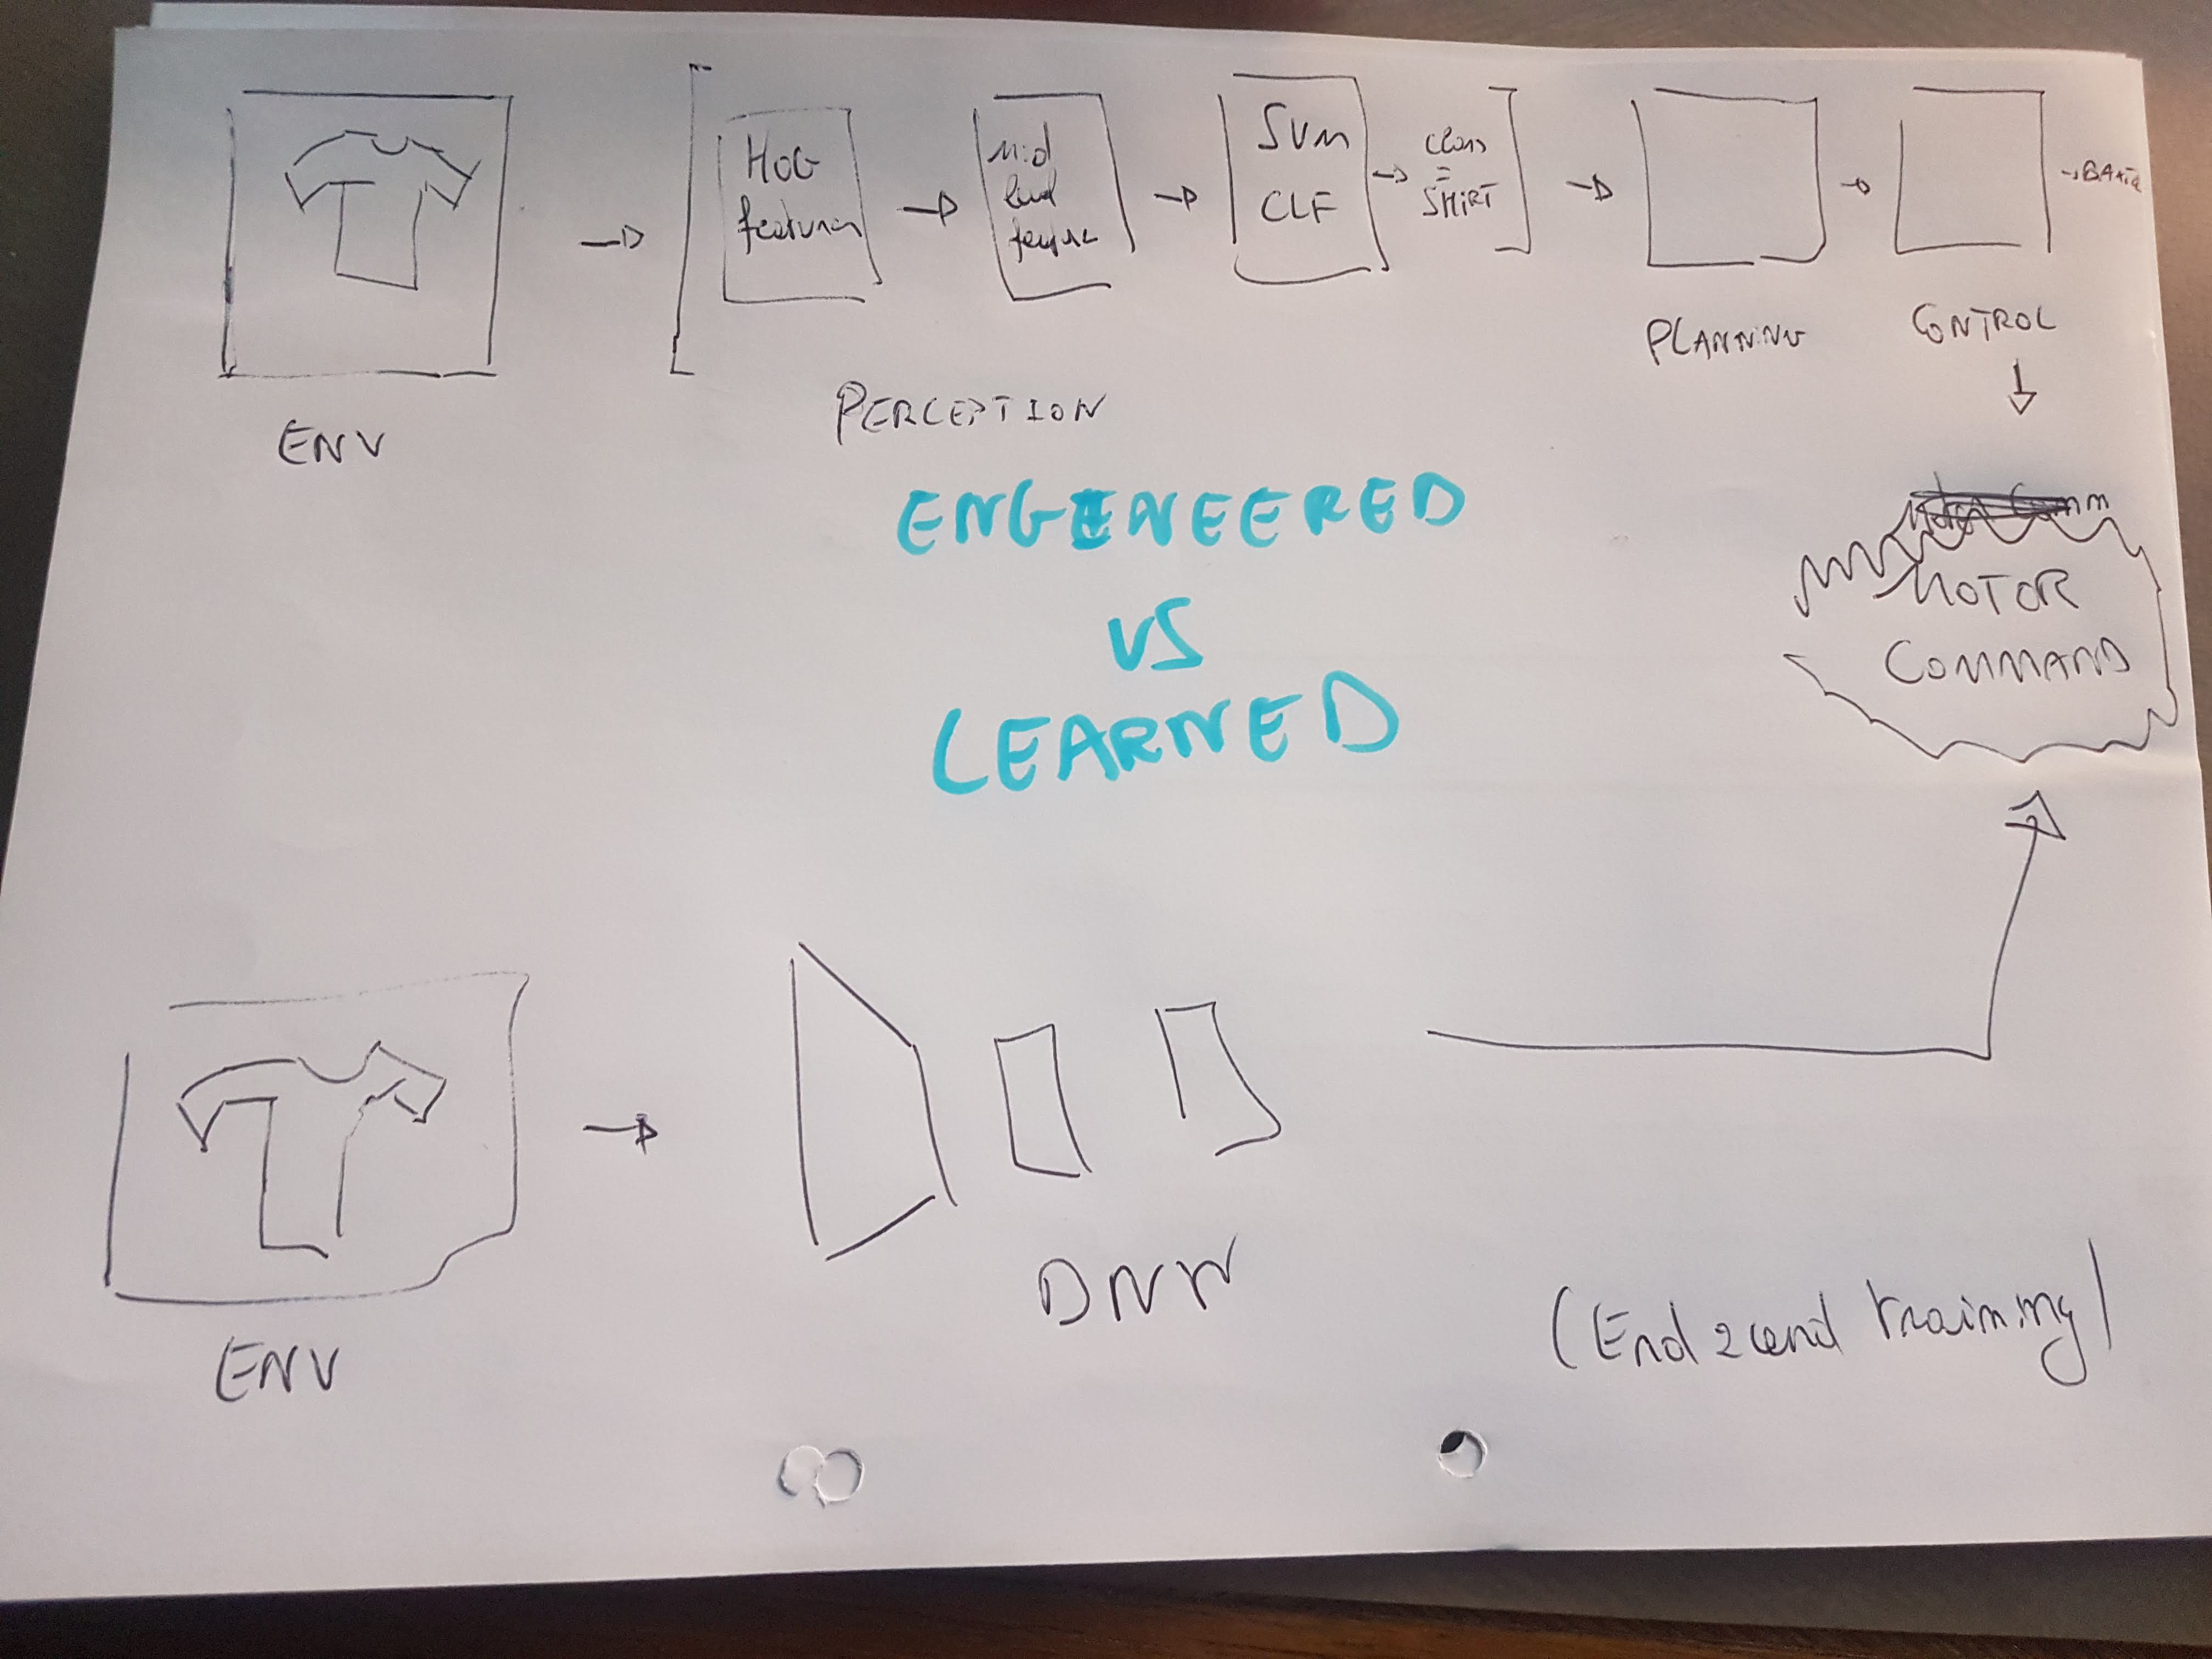
\includegraphics[width=\linewidth]{\home/chapters/01-introduction/figures/end2end-mockup}
    \caption{\textbf{Standard robotic control pipelines versus end-to-end architectures.} The diagram on the top shows how an image is processed to manually tuned features in order to do state estimation. This is then used downstream for trajectory planning and motor control. The diagram on the bottom shows an end-to-end approach to the same problem: an image is given to a deep neural network that learns its own features and executes actions directly on the actuators.}
    \label{fig:intro_end2end}
\end{figure}

\section{Robotic learning}
Machine learning introduction:
    - positioning ML %(cfr https://www.cs.cmu.edu/~tom/pubs/MachineLearning.pdf)
    - success applications: ML is preferred approach for MLP, speech recognition and computer vision , ... 
    - What is ML fundamentally. Definition. What does ML hopes to achieve ultimately? 
    - What is holding ML back in robotics? 
        Datasets, sample-efficient learning, weak or undefined learning signals 
        * a note on hardware debt.
    - DL History    (zie [2017[Deep learning in robotics: a review of recent research)
        * Linear regression has paved the way 
        * Activation functions allowed LR to deal with nonlinearities. Introduces biological similarities. 
        * Stacking layers of nonlinear models and find a way to train them
        * Robotics jumped on this in the 1980s.
        * GPUs came along for training together with large datasets. 


Process of doing robotic laundry is visualized in Figure~\ref{fig:intro_ml_flow}.
\pgfdeclarelayer{edgelayer}
\pgfdeclarelayer{nodelayer}
\pgfdeclarelayer{subnodelayer}

\pgfsetlayers{edgelayer,nodelayer,subnodelayer,main}

\tikzstyle{block} = [rectangle, draw, fill=blue!15, text width=8.0em, minimum height=1cm, text centered, rounded corners]
\tikzstyle{endBlock} = [circle, draw, fill=blue!15, text width=5.0em, minimum height=1cm, text centered, rounded corners]
\tikzstyle{empty} = [diamond, draw, fill=green!5, text width=7.5em, text centered]
\tikzstyle{line} = [draw, -latex']

\begin{figure}[htbp!]
\centering

\begin{tikzpicture}[auto, node distance=1.5cm, align=center]
  	\begin{pgfonlayer}{nodelayer}
  	
	\node [block] (data) {Training set};	
	\node [block, below of=data, yshift=-1cm] (algo) {Learning algorithm};
	\node [endBlock, below of=algo, yshift=-1cm] (h) {model};
	\node [left of=h, xshift=-2cm] (x) {input};
	\node [right of=h, xshift=2cm] (y) {output};

    \end{pgfonlayer}
        
   	\begin{pgfonlayer}{edgelayer}
	
	\path [line, thick] (data) -- (algo);
	\path [line, thick] (algo) -- (h);
	\path [line, thick] (x) -- (h);
	\path [line, thick] (h) -- (y);


    \end{pgfonlayer}
\end{tikzpicture}

\caption{\textbf{ML flow.}}
\label{fig:intro_ml_flow}
\end{figure}

Self-supervised dollar bill inspiration from Epstein in 2016.



\section{Accelerating robotic learning}
\subsection{Datasets}
\subsection{Simulation}
\subsection{Instrumentation}
\section{From behavioral cloning to understanding task intent}
\section{Research contributions} \label{sec:intro_contributions}
\begin{itemize}
    \item Dataset with people folding clothing
    \item Unsupervised reward function
    \item Low-cost robot setup to fold cloth invivo
    \item Instrumentation
    \item Gripper for folding
\end{itemize}

\section{Thesis structure}
This thesis is structured to first provide preliminary background and a review of the relevant literature. The remainder of the thesis deals with the methodology and results iterated in the previous Section~\ref{sec:intro_contributions}. The structure is as follows:
\begin{itemize}
    \item In Chapter~\ref{ch:lit}, we
\end{itemize}


\end{document}
